% per rivista https://www.atmospheric-measurement-techniques.net/

%% Copernicus Publications Manuscript Preparation Template for LaTeX Submissions
%% ---------------------------------
%% This template should be used for copernicus.cls
%% The class file and some style files are bundled in the Copernicus Latex Package, which can be downloaded from the different journal webpages.
%% For further assistance please contact Copernicus Publications at: production@copernicus.org
%% https://publications.copernicus.org/for_authors/manuscript_preparation.html

%% Please use the following documentclass and journal abbreviations for preprints and final revised papers.

%% 2-column papers and preprints
\documentclass[journal abbreviation, manuscript]{copernicus}
%\usepackage{color}


%% Journal abbreviations (please use the same for preprints and final revised papers)
% Advances in Geosciences (adgeo)
% Advances in Radio Science (ars)
% Advances in Science and Research (asr)
% Advances in Statistical Climatology, Meteorology and Oceanography (ascmo)
% Annales Geophysicae (angeo)
% Archives Animal Breeding (aab)
% ASTRA Proceedings (ap)
% Atmospheric Chemistry and Physics (acp)
% Atmospheric Measurement Techniques (amt)
% Biogeosciences (bg)
% Climate of the Past (cp)
% DEUQUA Special Publications (deuquasp)
% Drinking Water Engineering and Science (dwes)
% Earth Surface Dynamics (esurf)
% Earth System Dynamics (esd)
% Earth System Science Data (essd)
% E&G Quaternary Science Journal (egqsj)
% European Journal of Mineralogy (ejm)
% Fossil Record (fr)
% Geochronology (gchron)
% Geographica Helvetica (gh)
% Geoscience Communication (gc)
% Geoscientific Instrumentation, Methods and Data Systems (gi)
% Geoscientific Model Development (gmd)
% History of Geo- and Space Sciences (hgss)
% Hydrology and Earth System Sciences (hess)
% Journal of Bone and Joint Infection (jbji)
% Journal of Micropalaeontology (jm)
% Journal of Sensors and Sensor Systems (jsss)
% Magnetic Resonance (mr)
% Mechanical Sciences (ms)
% Natural Hazards and Earth System Sciences (nhess)
% Nonlinear Processes in Geophysics (npg)
% Ocean Science (os)
% Primate Biology (pb)
% Proceedings of the International Association of Hydrological Sciences (piahs)
% Scientific Drilling (sd)
% SOIL (soil)
% Solid Earth (se)
% The Cryosphere (tc)
% Weather and Climate Dynamics (wcd)
% Web Ecology (we)
% Wind Energy Science (wes)


\usepackage{todonotes}
\usepackage{hyperref}
\usepackage{graphicx}
\graphicspath{ {./img/} }

%% \usepackage commands included in the copernicus.cls:
%\usepackage[english]{babel}
%\usepackage{tabularx}
%\usepackage{cancel}
%\usepackage{multirow}
%\usepackage{supertabular}
%\usepackage{algorithmic}
%\usepackage{algorithm}
%\usepackage{amsthm}
%\usepackage{float}
%\usepackage{subfig}
%\usepackage{rotating}




\begin{document}

\title{Applying/Using Random Forest to separate meteorological and traffic influence from air quality measurement...} %migliorare


% \Author[affil]{given_name}{surname}

\Author[1]{Andrea Mario}{Trentini}
\Author[1]{Marco}{Belotti}
%\Author[]{}{}

\affil[1]{Università degli Studi di Milano - Via Celoria, 18 - 20133 MILANO - ITALY}

%% The [] brackets identify the author with the corresponding affiliation. 1, 2, 3, etc. should be inserted.

%% If an author is deceased, please mark the respective author name(s) with a dagger, e.g. "\Author[2,$\dag$]{Anton}{Aman}", and add a further "\affil[$\dag$]{deceased, 1 July 2019}".

%% If authors contributed equally, please mark the respective author names with an asterisk, e.g. "\Author[2,*]{Anton}{Aman}" and "\Author[3,*]{Bradley}{Bman}" and add a further affiliation: "\affil[*]{These authors contributed equally to this work.}".


\correspondence{Andrea Mario Trentini (andrea.trentini@unimi.it)}

\runningtitle{TEXT}

\runningauthor{TEXT}





\received{}
\pubdiscuss{} %% only important for two-stage journals
\revised{}
\accepted{}
\published{}

%% These dates will be inserted by Copernicus Publications during the typesetting process.


\firstpage{1}

\maketitle


\tableofcontents

\listoftodos




\begin{abstract}
ABSTRACT
\end{abstract}


%\copyrightstatement{TEXT} %% This section is optional and can be used for copyright transfers.


\introduction  %% \introduction[modified heading if necessary]


\begin{figure}
\centering
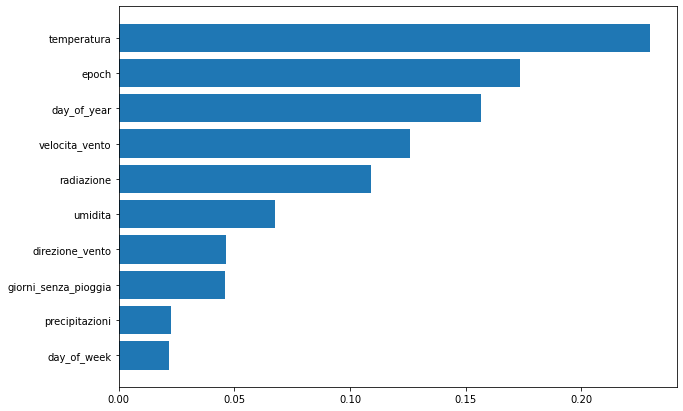
\includegraphics[width=0.75\textwidth]{intro_importanza_totale}
\caption{Media delle importanze delle variabili predittrici nei modelli generati durante le nostre analisi}
\label{fig:importanza_tot}
\end{figure}

\todo{contesto aria lombardia}

\todo{trend **storici**, mancano i grafici}

\todo{riprendere da capitolo 3 della tesi, ma solo le parti che ancora non includono le relazioni fra le varie variabili}

\todo{contestare la percezione (articolo rapporto EU)}

\todo{rete misurazione ARPA}

\todo{scopo: scorporare grande variazione causata dal meteo per evidenziare cambiamenti nel quadro emissivo}

\todo{ulteriore: periodo COVID e influenza del traffico sull'inquinamento, areac}

\todo{carrellata delle variabili che sono state prese in considerazione}



\todo{tradurre e sintetizzare}


L'inquinamento atmosferico è un tema che viene spesso discusso e dibattuto, visto che respirare un'aria pulita è considerato un requisito basilare per la buona salute umana. Da anni il WHO \cite{world2006air} si occupa di studiare i potenziali effetti dell'inquinamento sulla salute umana, cercando di stimare che tipo di impatto possa avere un'esposizione prolungata ad alte concentrazioni.  

Chiaramente non è facile riuscire a stabilire con certezza il collegamento tra causa (esposizione agli inquinanti) ed effetto (malattie e morte) poiché spesso i danni si manifestano solo a seguito di ripetute e prolungate esposizioni, così come non è facile riuscire a stabilire con certezza che una morte sia stata causata esplicitamente dall'inquinamento atmosferico.  

L'inquinamento atmosferico è un fenomeno molto complicato da analizzare, poiché sia per quanto riguarda la produzione e l'emissione in atmosfera che per la dispersione entrano in gioco molti fenomeni e fattori, che hanno scale spaziali molto differenti e che è difficile riuscire ad analizzare correttamente.  

Se in alcune zone del mondo, soprattutto quelle dei paesi in forte via di sviluppo come il sud-est asiatico o l'India, l'inquinamento rappresenta ancora un problema molto grave causato dall'aumento del fabbisogno energetico che è stato soddisfatto incrementando l'uso di combustibili fossili, in Europa (come in altre parti del mondo) negli ultimi 25 anni si è registrato un disaccoppiamento tra la crescita economica e le emissioni dei principali inquinanti, causato da un maggiore impegno nel loro contenimento da parte dei governi, che hanno imposto limitazioni e misure sempre più stringenti \cite{cattani2014analisi}.

È quindi normale che sia la comunità scientifica che le autorità incaricate di decidere le misure di contenimento da mettere in campo siano interessate a capire quale sia il reale andamento delle concentrazioni di inquinanti, cercando di identificare quali possano essere i metodi più efficaci e quanto le variazioni registrate siano attribuibili specificatamente ai cambiamenti delle emissioni umane rispetto agli effetti di altri fattori come il clima che possono avere un'influenza molto maggiore sulle concentrazioni registrate \cite{porter2001ozone}.  

Quasi tutti gli inquinanti di maggior interesse, come gli ossidi di azoto, il biossido di zolfo, il monossido di carbonio, il particolato e l'ozono sono infatti caratterizzati da una forte variabilità stagionale che, per esempio, non ci permette di confrontare valori registrati durante la stagione estiva con quelli invernali, così come l'azione di agenti atmosferici come il vento e la pioggia possono portare ad abbattimenti delle concentrazioni. Nella pianura padana, per esempio, è infatti frequente assistere, specialmente nei mesi invernali che sono già quelli più critici per le concentrazioni di molti inquinanti, a lunghi periodi senza precipitazioni che portano a grossi aumenti delle concentrazioni, che però vengono rapidamente abbattute all'arrivo della pioggia.   

Per poter quindi trarre delle conclusioni oggettive sullo stato della qualità dell'aria, riuscendo ad identificare le cause delle variazioni che si registrano e quindi a capire anche l'efficacia delle misure prese, nel corso degli ultimi anni molti studi si sono avvalsi di diverse tecniche statistiche/probabilistiche per poter fare un'analisi oggettiva sugli andamenti dell'inquinamento atmosferico \cite{cattani2014analisi,rao1994detecting,libiseller2005meteorological,pbl2010trends}.
%\todo{atrent: potrebbe valer la pena riportare alcuni concetti dai paper citati?
%marco: vedi frase sotto}
In tutti gli studi si è evidenziato come considerare anche la meteorologia durante l'analisi delle concentrazioni degli inquinanti, cercando di eliminarne l'influenza, sia fondamentale per poter capire come dei cambiamenti nel quadro emissivo vengano riflessi sulle concentrazioni misurate. Questo poi ci permette di poter fare delle analisi oggettive e quantitative più precise sui trend delle serie storiche, qualsiasi sia la località considerata, visto che i metodi utilizzati sono facilmente generalizzabili allo scenario che si vuole considerare in ogni analisi specifica. 

Riuscire ad avere a disposizione tecniche e modelli che ci permettono di analizzare l'andamento delle concentrazioni e ad identificare le cause che possono cambiare questo andamento ci permette di capire quali siano le aree più critiche su cui andare ad intervenire ma ci può anche permettere di identificare gli interventi più efficaci e sui quali conviene investire maggiormente. La crescita economica e l'aumento del fabbisogno energetico rendono quindi fondamentale il controllo delle emissioni, per poter mantenere la qualità dell'aria a livelli non pericolosi per la salute umana e al tempo stesso non bloccare le attività economiche.  

Qualsiasi studio sui trend degli inquinanti, così come qualsiasi conclusione che ne può derivare, non possono quindi non tener conto degli effetti della meteorologia sulle concentrazioni, poiché i risultati che si otterrebbero correrebbero il rischio di non rappresentare il cambiamento nelle emissioni antropiche ma anche una variazione nei fenomeni atmosferici e negli agenti climatici.  

Il nostro obbiettivo è quindi stato quello di ricercare una tecnica per normalizzare i dati sull'inquinamento rispetto alla meteorologia e al clima, ovvero che fosse in grado di eliminare l'influenza degli agenti atmosferici come pioggia, vento e radiazione solare e della stagionalità che porta ad avere condizioni più o meno favorevoli alla dispersione dalle concentrazioni registrate degli inquinanti, in modo da arrivare poi ad avere una serie storica su cui poter fare analisi sull'efficacia delle misure prese nel corso degli anni per il contenimento delle concentrazioni.  

Un metodo comune per riuscire a fare questa ``pulizia''%\todo{atrent: le virgolette si fanno così} 
dei dati si basa sulla creazione di modelli statistici che tramite l'uso di diverse variabili \textit{predittrici}
%\todo{atrent: andrà spiegato bene cosa si intende col termine, qui lo metterei tra virgolette o in corsivo
%marco: predittrici è il nome formale delle variabili nei modelli statistici
%atrent: forse meglio citare/spiegare il termine ``proxy''
%marco: ho aggiunto una nuova frase che credo spieghi abbastanza bene il termine predittrici, non ho citato il termine proxy perchè la definizione statistica non corrisponde con quella di variabile predittrice}
, come le misure meteorologiche su vento, precipitazioni e radiazione solare e variabili temporali legate al giorno dell'anno e alla date, siano capaci di prevedere i valori delle concentrazioni che si sarebbero misurate per un inquinante in base ai valori di ciascuna. Col termine variabile predittrice, infatti, si intende una variabile in grado di spiegare, anche solo parzialmente, cambiamenti nel valore di un'altra variabile, permettendo quindi di fare previsioni su di esso basandosi sul valore della prima. Se i modelli che riusciamo a creare si rivelano abbastanza precisi nell'attività predittoria e in grado di spiegare buona parte della varianza delle concentrazioni allora possiamo usarli con una certa confidenza per eliminare gli effetti della meteorologia dalle concentrazioni di inquinanti.

% nota per me (atrent)
% step 1: trovare predittrici
% step 2: usarle per scorporare effetto

Questo procedimento viene però complicato dal fatto che le dinamiche che portano la meteorologia a modificare le concentrazioni varino molto a seconda della località e che quindi differenti contesti, come ad esempio possono essere una città rispetto ad una località montana o situata a fondo valle, necessitino trattazione specifiche a seconda del caso. Inoltre è chiaro come le variabili meteorologiche tra di loro siano collegate e correlate, cioè che cambiamenti nei valori di una vengano riflessi anche sulle altre, e questo porta all'insorgere di una serie di problemi come la normalità, la multi collinearità e l'indipendenza che rendono la trattazione con diversi metodi molto difficile e complicata \cite{gunst1975regression}. 
%\todo{atrent: spiegare i termini o citare biblio
%marco: aggiunta breve spiegazione più bib
%atrent: ottimo collegamento con introduzione del termine proxy sopra
%marco: non ho introdotto il termine proxy, ma comunque è spiegato cosa si intende quando si dice che i valori di una variabile influenzano quelli di un'altra}

Nel corso degli ultimi tre decenni nel mondo dell'informatica ha preso campo un'area detta \textit{machine learning} (ML)
%\todo{atrent: almeno un ref sul ML, anche un testo ufficiale o simili
%mbelotti: aggiunta ref}
, che fa uso dei computer e della statistica per creare dei modelli predittori che potessero porsi come alternativa ai classici metodi statistici già esistenti \cite{james2013introduction}. Sono quindi state sviluppate tecniche di ML non parametriche, ovvero che non necessitano di fare alcun tipo di assunzione statistica sulle variabili considerate, che, grazie all'uso dei computer per analizzare grosse moli di dati, permettono di arrivare alla creazione di modelli con buone capacità predittive anche senza occuparsi dei problemi che invece caratterizzano gli approcci puramente statistici. Questi ultimi richiedono infatti, prima di poterli applicare, di fare una serie di assunzioni
%\todo{quali?
%marco: specificato alcune delle assunzioni necessarie (le più semplici, perchè alcune richiederebbero una trattazione più specifica dell'argomento per essere introdotte) e aggiunto footnote} 
sui dati considerati, come la linearità della relazione con i valori della variabile da predirre o l'assenza di autocorrelazione\footnote{Per autocorrelazione si intende quel fenomeno per cui i valori di una variabile sono dipendenti dai valori assunti in precedenza dalla stessa}, e su quali siano le relazioni che li legano ed inoltre molte volte anche la matematica necessaria è complicata e richiede particolare attenzione nella trattazione per essere sicuri di ottenere dei risultati attendibili. Gli algoritmi di machine learning, invece, sfruttando la capacità computazionale degli elaboratori, permettono di arrivare ad ottenere dei modelli altrettanto affidabili senza però doversi preoccupare dei diversi aspetti richiesti dalla statistica e che spesso ne limitano l'applicabilità. Inoltre, molte volte, l'obbiettivo dei modelli statistici è quello di inferire il modello dei dati per il caso considerato, ovvero capire come diversi fattori influenzino quantitativamente i valori di una variabile di interesse, mentre nel machine learning l'obbiettivo principale solitamente è quello di essere capaci di fare previsioni precise sui valori di tale variabile in base a quelli dei diversi fattori considerati \cite{breiman2003statistical}. 
%\todo{atrent: spiegare per sommi capi differenza fra i modelli classici e il ML
%marco: aggiunta spiegazione più bib
%atrent: dettagliare un po' meglio
%marco: aggiunte due spiegazioni sui vantaggi del ML rispetto alla statistica, così mi sembra più chiaro}

ARPA Lombardia \footnote{\url{https://www.arpalombardia.it/Pages/ARPA_Home_Page.aspx}}
%\todo{atrent: link
%mbelotti: aggiunta footnote}
possiede, sul territorio regionale, una rete di 85 stazioni fisse che, per mezzo di analizzatori automatici, sono in grado di fornire rilevazioni ad intervalli di tempo regolari, permettendoci di creare quindi un dettagliato catalogo dei valori delle concentrazioni nel corso del tempo. Tutte queste rilevazioni vengono poi rese accessibili liberamente tramite archivi online, per permetterne la libera consultazione da parte di tutti i cittadini.  

Nel nostro studio abbiamo quindi fatto uso di questi dati, unitamente a quelli delle variabili meteorologiche sempre resi disponibili da ARPA Lombardia, per creare tramite l'uso di una tecnica di machine learning chiamata \textit{Random Forest} \cite{breiman2001random}
%\todo{atrent: link/ref
%mbelotti: aggiunta ref}
%\todo{atrent: quando introduci un termine fa messo in corsivo, specie se è inglese}
dei modelli predittivi che ci permettano di arrivare a fare questa normalizzazione delle concentrazioni di inquinanti rispetto alla meteorologia e quindi di analizzare come si sia evoluta la situazione nella nostra regione nel corso degli anni dal 2012 ad oggi, cercando di capire quali siano stati i provvedimenti e gli eventi più efficaci nell'abbattimento delle concentrazioni.  

%Nel capitolo 2 viene introdotto Random Forest e viene mostrato come questa tecnica possa essere utilizzata per eliminare gli effetti della meteorologia e della stagionalità dall'andamento delle concentrazioni.  

%Nel capitolo 3 viene analizzata, utilizzando la tecnica appena discussa, la situazione regionale andando a controllare l'andamento delle serie dei principali inquinanti nei capoluoghi di provincia lombardi.  

%Nel capitolo 4 verranno presentate le analisi svolte sull'influenza del traffico sulle concentrazioni di tre inquinanti: ossidi di azoto, particolato atmosferico (PM10 e PM2.5) e monossido di carbonio.

%Nel capitolo 5 verrà presentata un'analisi del periodo di diffusione dell'epidemia di Covid-19 e di quali siano stati gli effetti del conseguente \textit{lockdown} svoltosi nei mesi di marzo ed aprile sulle concentrazioni.















%%%%%%%%%%%%%%%%%%%%%%%%%%%%%%%%%%%%%%%%%%%%%%%%%%%%%%%%

\section{State of the art}

lavori simili

approfondimento da introduzione

inventario INEMAR ecc.

trend ecc.


%%%%%%%%%%%%%%%%%%%%%%%%%%%%%%%%%%%%%%%%%%%%%%%%%%%%%%%%
\section{rete misurazione ARPA}

centraline

mappa delle centraline, indicare tutti i sensori usati nelle analisi

modalità scaricamento (se ci sta dire del problema webstacles, hanno liberato i dati solo recentemente)

scelta delle centraline su cui lavorare

descrizione dei dati





%%%%%%%%%%%%%%%%%%%%%%%%%%%%%%%%%%%%%%%%%%%%%%%%%%%%%%%%
\section{Random Forest e applicazione ai dati in oggetto}

con snippet di (pseudo)codice

\subsection{random forest}
intro random forest (perché zero results sulla rivista)

\todo{prendere da "Normalizzazione meteorologica utilizzando Random Forest", fare molti tagli ma la sostanza ok}


come è stata fatta applicazione ai dati


\subsection{qualità dei modelli}

affidabilità

importanza variabili

\subsection{risultati: scorporo meteo}

\subsubsection{$NO_x$ e $NO_2$}
\subsubsection{PM10 e PM2.5}
\subsubsection{CO}
\subsubsection{Ozono}
\subsubsection{Ammoniaca}
\subsubsection{Benzene}
\subsubsection{$SO_2$}



\subsection{risultati: scorporo traffico (areac)}
\subsubsection{$NO_x$ e $NO_2$}
\subsubsection{CO}
\subsubsection{PM10}



\subsection{risultati: periodo COVID}
\subsubsection{$NO_x$ e $NO_2$}
\subsubsection{PM10 e PM2.5}
\subsubsection{CO}
\subsubsection{Ozono}
\subsubsection{Ammoniaca}
\subsubsection{Benzene}
\subsubsection{$SO_2$}



\conclusions  %% \conclusions[modified heading if necessary]
riassunto conclusioni

critica all'articolo vergognoso, specie in termini di previsioni del modello fuori dai periodi di training (col tempo che passa)

%% The following commands are for the statements about the availability of data sets and/or software code corresponding to the manuscript.
%% It is strongly recommended to make use of these sections in case data sets and/or software code have been part of your research the article is based on.

\codeavailability{url repo git} %% use this section when having only software code available


%\dataavailability{TEXT} %% use this section when having only data sets available


%\codedataavailability{url repo git} %% use this section when having data sets and software code available


%\sampleavailability{TEXT} %% use this section when having geoscientific samples available


%\videosupplement{TEXT} %% use this section when having video supplements available


%\appendix
%\section{}    %% Appendix A
%\subsection{}     %% Appendix A1, A2, etc.
%\noappendix       %% use this to mark the end of the appendix section. Otherwise the figures might be numbered incorrectly (e.g. 10 instead of 1).

%% Regarding figures and tables in appendices, the following two options are possible depending on your general handling of figures and tables in the manuscript environment:

%% Option 1: If you sorted all figures and tables into the sections of the text, please also sort the appendix figures and appendix tables into the respective appendix sections.
%% They will be correctly named automatically.

%% Option 2: If you put all figures after the reference list, please insert appendix tables and figures after the normal tables and figures.
%% To rename them correctly to A1, A2, etc., please add the following commands in front of them:

\appendixfigures  %% needs to be added in front of appendix figures

\appendixtables   %% needs to be added in front of appendix tables

%% Please add \clearpage between each table and/or figure. Further guidelines on figures and tables can be found below.



\authorcontribution{AUTHORCONTRIB} %% this section is mandatory

\competinginterests{Authors declare no competing interests.} %% this section is mandatory even if you declare that no competing interests are present

\disclaimer{DISCLAIMER} %% optional section

\begin{acknowledgements}
ACK
\end{acknowledgements}



%% REFERENCES
%% The reference list is compiled as follows:
%\begin{thebibliography}{}
%\bibitem[AUTHOR(YEAR)]{LABEL1}
%REFERENCE 1
%\bibitem[AUTHOR(YEAR)]{LABEL2}
%REFERENCE 2
%\end{thebibliography}

%% Since the Copernicus LaTeX package includes the BibTeX style file copernicus.bst,
%% authors experienced with BibTeX only have to include the following two lines:
%%
\bibliographystyle{copernicus}
\bibliography{Biblio.bib}
%%
%% URLs and DOIs can be entered in your BibTeX file as:
%%
%% URL = {http://www.xyz.org/~jones/idx_g.htm}
%% DOI = {10.5194/xyz}


%% LITERATURE CITATIONS
%%
%% command                        & example result
%% \citet{jones90}|               & Jones et al. (1990)
%% \citep{jones90}|               & (Jones et al., 1990)
%% \citep{jones90,jones93}|       & (Jones et al., 1990, 1993)
%% \citep[p.~32]{jones90}|        & (Jones et al., 1990, p.~32)
%% \citep[e.g.,][]{jones90}|      & (e.g., Jones et al., 1990)
%% \citep[e.g.,][p.~32]{jones90}| & (e.g., Jones et al., 1990, p.~32)
%% \citeauthor{jones90}|          & Jones et al.
%% \citeyear{jones90}|            & 1990



%% FIGURES

%% When figures and tables are placed at the end of the MS (article in one-column style), please add \clearpage
%% between bibliography and first table and/or figure as well as between each table and/or figure.

% The figure files should be labelled correctly with Arabic numerals (e.g. fig01.jpg, fig02.png).


%% ONE-COLUMN FIGURES

%%f
%\begin{figure}[t]
%\includegraphics[width=8.3cm]{FILE NAME}
%\caption{TEXT}
%\end{figure}
%
%%% TWO-COLUMN FIGURES
%
%%f
%\begin{figure*}[t]
%\includegraphics[width=12cm]{FILE NAME}
%\caption{TEXT}
%\end{figure*}
%
%
%%% TABLES
%%%
%%% The different columns must be seperated with a & command and should
%%% end with \\ to identify the column brake.
%
%%% ONE-COLUMN TABLE
%
%%t
%\begin{table}[t]
%\caption{TEXT}
%\begin{tabular}{column = lcr}
%\tophline
%
%\middlehline
%
%\bottomhline
%\end{tabular}
%\belowtable{} % Table Footnotes
%\end{table}
%
%%% TWO-COLUMN TABLE
%
%%t
%\begin{table*}[t]
%\caption{TEXT}
%\begin{tabular}{column = lcr}
%\tophline
%
%\middlehline
%
%\bottomhline
%\end{tabular}
%\belowtable{} % Table Footnotes
%\end{table*}
%
%%% LANDSCAPE TABLE
%
%%t
%\begin{sidewaystable*}[t]
%\caption{TEXT}
%\begin{tabular}{column = lcr}
%\tophline
%
%\middlehline
%
%\bottomhline
%\end{tabular}
%\belowtable{} % Table Footnotes
%\end{sidewaystable*}
%
%
%%% MATHEMATICAL EXPRESSIONS
%
%%% All papers typeset by Copernicus Publications follow the math typesetting regulations
%%% given by the IUPAC Green Book (IUPAC: Quantities, Units and Symbols in Physical Chemistry,
%%% 2nd Edn., Blackwell Science, available at: http://old.iupac.org/publications/books/gbook/green_book_2ed.pdf, 1993).
%%%
%%% Physical quantities/variables are typeset in italic font (t for time, T for Temperature)
%%% Indices which are not defined are typeset in italic font (x, y, z, a, b, c)
%%% Items/objects which are defined are typeset in roman font (Car A, Car B)
%%% Descriptions/specifications which are defined by itself are typeset in roman font (abs, rel, ref, tot, net, ice)
%%% Abbreviations from 2 letters are typeset in roman font (RH, LAI)
%%% Vectors are identified in bold italic font using \vec{x}
%%% Matrices are identified in bold roman font
%%% Multiplication signs are typeset using the LaTeX commands \times (for vector products, grids, and exponential notations) or \cdot
%%% The character * should not be applied as mutliplication sign
%
%
%%% EQUATIONS
%
%%% Single-row equation
%
%\begin{equation}
%
%\end{equation}
%
%%% Multiline equation
%
%\begin{align}
%& 3 + 5 = 8\\
%& 3 + 5 = 8\\
%& 3 + 5 = 8
%\end{align}
%
%
%%% MATRICES
%
%\begin{matrix}
%x & y & z\\
%x & y & z\\
%x & y & z\\
%\end{matrix}
%
%
%%% ALGORITHM
%
%\begin{algorithm}
%\caption{...}
%\label{a1}
%\begin{algorithmic}
%...
%\end{algorithmic}
%\end{algorithm}
%
%
%%% CHEMICAL FORMULAS AND REACTIONS
%
%%% For formulas embedded in the text, please use \chem{}
%
%%% The reaction environment creates labels including the letter R, i.e. (R1), (R2), etc.
%
%\begin{reaction}
%%% \rightarrow should be used for normal (one-way) chemical reactions
%%% \rightleftharpoons should be used for equilibria
%%% \leftrightarrow should be used for resonance structures
%\end{reaction}
%
%
%%% PHYSICAL UNITS
%%%
%%% Please use \unit{} and apply the exponential notation


\end{document}












%intro veramente oscena
%
%"increasingly worsening" in realtà è esattamente il contrario
%
%"4.6 million people die each year from causes directly attributable to air pollution [2]" invece sono morti PREMATURE (è già nel titolo del paper citato!) mentre i "car crashes" sono morti vere!
%
%non c'entra inoltre NULLA il climate change che non è dovuto all'inquinamento ma semmai alla CO2 (che NON è un inquinante)
%
%i costi indicati per le stazioni di monitoraggio sono BASSISSIMI per una PA che voglia gestire una rete di sensori, si tratta in fondo di qualche centinaio di stazioni per regione!
%
%"vehicle" non è vero, come molti studi stanno dimostrando e come molti rapporti ufficiali (citare ARPA ecc.) stanno verbalizzando, la quota parte del traffico è ormai molto ridotta e difficilmente comprimibile come ha dimostrato il lockdown
%
%lo state of the art lo possiamo copiare parzialmente, citando correttamente i findings, non come fanno loro!
%
%loro fanno "As a case study, we combine three years of sensor and vehicle logs from the city of Milan, from 2013 to 2016", noi arriviamo fino al 2020
%
%copiamo anche la struttura, che cmq è standard
%
%noi usiamo i dati di tutta la regione e su uno span più ampio
%
%e, IMPORTANTE, noi prendiamo in considerazione il lockdown in cui si vede che cambia poco o nulla!!!
%
%vale la pena fare lo smoothing dei dati che hanno fatto loro?
%
%temperature risulta anche a loro
%
%figure 3, euro4 peggiore di euro0 su PM10?
%
%cosa vuol dire "authorized" vs. "non authorized"?!? indagare tutta la correlation matrix
%
%noi forniamo il sw usato, gli script, loro NO
%
%inoltre non citano un singolo url di un dataset!!!
%
%la descrizione della macchina è inutile e ininfluente, specie se non fornisci il tuo software
%
%plottare il CAQI nel corso degli anni per dimostrare che scende/sale
%
%conclusioni nostre (da tesi), data come predittore, ergo poco legato ad altri fattori, non si può NON avere sensori perché la situazione cambia nel tempo (tecnologie cambiano, MIGLIORANO, vedi grafici negli anni)
